%! TEX root = main.tex

In our case study, we compared the results of PINNs against our in-house CFD solver, PetIBM.
It is necessary to verify and validate both the PINN solver and PetIBM.
The verification was done with the 2D Taylor-Green vortex (TGV) at Reynolds number $Re=\num{100}$, and the validation case was the 2D cylinder flow at $Re=40$.
Once the verification and validation were done, we carried out the case study of the 2D cylinder flow at $Re=\num{200}$, which exhibits vortex shedding.

\subsection{Verification: 2D Taylor-Green Vortex (TGV), $Re=\num{100}$}

The 2D TGV problems with periodic boundary conditions have closed-form analytical solutions; hence, they usually serve as standard verification cases for CFD solvers. 
We used the following 2D Taylor-Green vortex, which corresponds to $Re=\num{100}$, to verify both the PINN solver and PetIBM:
\begin{equation}\label{eq:tgv}
    \left\{
        \begin{aligned}
            u(x, y, t) &= \cos(x)\sin(L)\exp(-2 \nu t) \\
            v(x, y, t) &= - \sin(x)\cos(y)\exp(-2 \nu t) \\
            p(x, y, t) &= -\frac{1}{4}\left(\cos(2x) + \cos(2y)\right)\exp(-4 \nu t)
        \end{aligned}
    \right.
\end{equation}
where $\nu$ is the kinematic viscosity;
$x$ and $y$ represent the spatial coordinates in the domain of $\left[-\pi, \pi\right]\times\left[-\pi, \pi\right]$;
$t \in [0, 100]$ is the simulation time;
$u$ and $v$ denote the velocity components in the $x$ and $y$ directions;
$p$ is the pressure.
The periodic conditions are applied to all boundaries.

In PetIBM, we used the Adams-Bashforth and the Crank-Nicolson schemes for the temporal discretization in convection and diffusion, respectively.
The spatial discretization was central difference for all terms.
Therefore, we expected to see a second-order convergence in both time and space for this 2D TGV problem.
Here we use the following $L_2$ spatial-temporal error to examine the convergence:
\begin{equation}\label{eq:spt-err-def}
    \begin{aligned}
    L_{2,sp-t} \equiv &\sqrt{
        \frac{1}{L_x L_y T}
        \iiint\limits_{x, y, t} \lVert f - f_{ref} \rVert^2 \diff x \diff y \diff t
    } \\
    = &
    \sqrt{\frac{1}{N_x N_y N_t}\sum\limits_{i=1}^{N_x}\sum\limits_{j=1}^{N_y}\sum\limits_{k=1}^{N_t}\left(f^{(i, j, k)} - f_{ref}^{(i, j, l)}\right)^2}
    \end{aligned}
\end{equation}
$N_x$, $N_y$, and $N_t$ represent the number of cells in $x$, $y$, and $t$;
$L_x$ and $L_y$ are the domain lengths in $x$ and $y$;
$T$ is the total simulation time;
$f$ is the flow quantity of our interest, while $f_{ref}$ is the corresponding analytical solution.
The superscript $(i, j, k)$ denotes the value at the $(i, j, k)$ point in the discretized spatial-temporal space.
The characteristic cell size in a spatial-temporal sense is simply $\sqrt[3]{\frac{1}{N_x N_y N_t}}$, meaning the characteristic number of cells is $\sqrt[3]{N_x N_y N_t}$.

In PetIBM verification, we ran simulations with $2^{n} \times 2^{n}$ cells for $i=4$, $5$, $\dots$, $10$.
The time step size $\Delta t$ did not follow a fixed refinement ratio, and they were $\Delta t = \num{1.25e-1}$, $\num{8e-2}$, $\num{4e-2}$, $\num{2e-2}$, $\num{1e-2}$, $\num{5e-3}$, and $\num{1.25e-3}$, respectively.
$\Delta t$ was determined based on the maximum allowed CFL number and whether it was a factor of $2$ (to output transient results every $\num{2}$ simulation seconds).
The velocity and pressure systems were both solved with BiCGSTAB (biconjugate gradient stabilized method).
The velocity systems used a block Jacobi preconditioner, and the pressure system used an algebraic multigrid preconditioner from NIVIDA's AmgX library.
At each time step, both solvers stopped when preconditioned residual reached $\num{1e-14}$.
The hardware contains 5 physical cores of Intel E5-2698 v4 and 1 V100 GPU.

\begin{figure}
    \centering%
    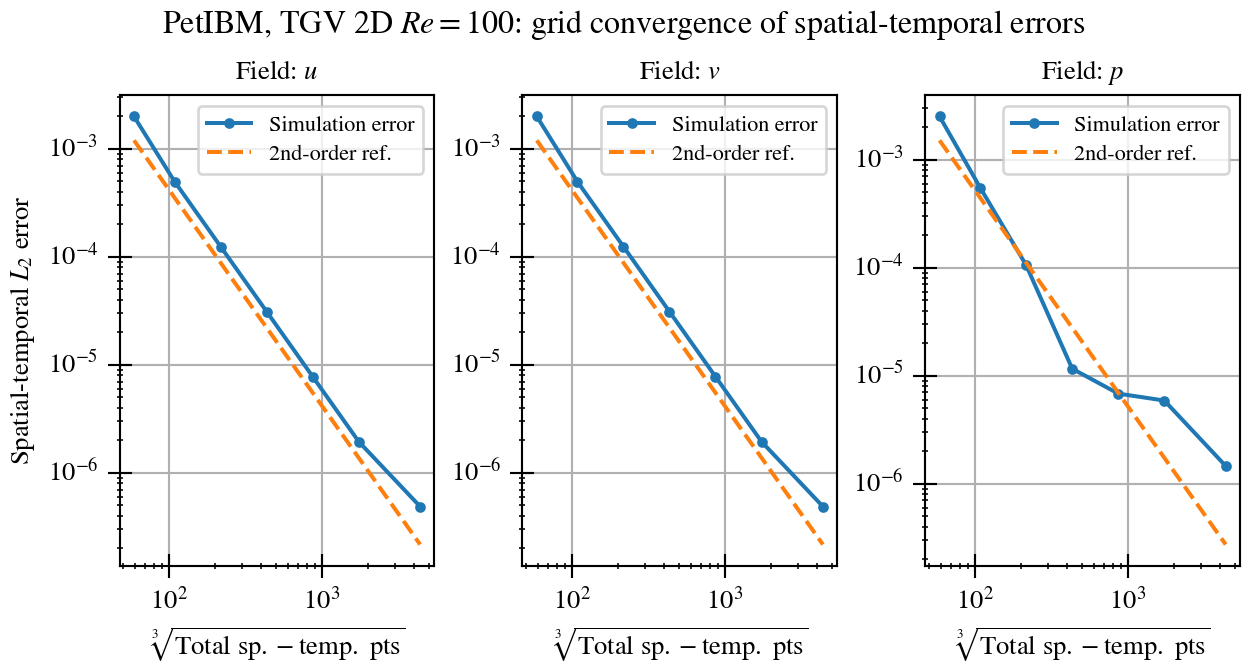
\includegraphics[width=\columnwidth]{tgv-2d-re100/petibm-tgv-2d-re100-convergence}%
    \caption{%
        Grid-convergence test of 2D TGV $Re=\num{100}$ w/ PetIBM
    }
    \label{fig:tgv-petibm-convergence}%
\end{figure}

Figure \ref{fig:tgv-petibm-convergence} shows the spatial-temporal convergence results of PetIBM.
Both $u$ and $v$ follow an expected second-order convergence before the machine round-off errors dominates at the $1024 \times 1024$ grid.
However, the pressure field does not follow such a perfect convergence pattern.
After scrutinization, we found the cause was that AmgX did not solve the pressure systems to the tolerance we defined.
NVIDIA's AmgX has a hard-coded stop mechanism when relative preconditioned residuals (relative to the initial residual) reach the machine precision.
So while we configured the absolute tolerance to be $1\times 10^{-14}$, the final preconditioned residuals of the pressure systems did not match this value.
On the other hand, the velocity systems were solved to the requested tolerance.
In sum, we considered the verification of PetIBM to be successful because the convergence anomaly in pressure was irrelevant to the code implementation in PetIBM.

Next we solved this TGV problem with the PINN solver.
The optimization was done with PyTorch's Adam optimizer with $\beta_1=\num{0.9}$, $\beta_2=\num{0.999}$, and $\epsilon=\num{10e-8}$.
The total number of optimization iteration was fixed to \num{400000}.
Two learning rate schedulers were tested for our curiosity: the exponential learning rate and the cyclical learning rate.
Both were also implemented in PyTorch.
The exponential learning rate followed this formula: $\operatorname{lr}(iter) = 0.95^\frac{iter}{5000}$, where $iter$ denotes the iteration counter during optimization.
The cyclical learning rate schedulers was configured with $\eta_{low}=\num{1.5e-5}$, $\eta_{high}=\num{1.5e-3}$, $N_c=\num{5000}$, and $\gamma=\num{0.999989}$.
These values are chosen so that the peak learning rate of each cycle is a just slightly higher than the exponential learning rate.
In the figure legends, the exponential learning rate will be simply denoted as {\it Exponential}, while the cyclical learning rate is {\it Cyclical}.
Figure \ref{fig:tgv-learning-rate-hist} shows a comparison of the two learning rate schedulers.

\begin{figure}
    \centering%
    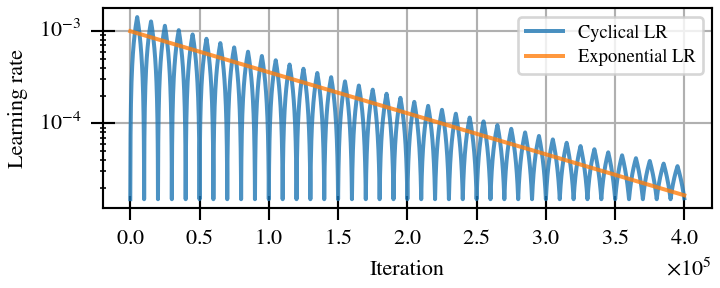
\includegraphics[width=\columnwidth]{tgv-2d-re100/learning-rate-hist}%
    \caption{%
        Learning-rate history of 2D TGV $Re=\num{100}$ w/ PINN
    }
    \label{fig:tgv-learning-rate-hist}%
\end{figure}

The MLP neural network consisted of \num{3} hidden layers and \num{128} neurons per layer.
A total number of \num{81920000} spatial-temporal points were used to evaluate the PDE losses (i.e., the $L_1$, $L_2$, and $L_3$ in figure \ref{fig:pinn-workflow}).
These spatial-temporal points were randomly sampled from $x,y \in \left[-\pi, \pi\right]$ and $t \in \left(0, 100\right]$.
(Note that $t=0$ is excluded.)
In each optimization iteration, only \num{8192} points were used to evaluate the PDE losses, meaning the optimization would see each point \num{40} times because we have a total of \num{400000} iterations.
Similarly, \num{81920000} spatial-temporal points were sampled from $x,y \in \left[-\pi, \pi\right]$ and $t=0$ for the initial condition loss (i.e., $L_4$ to $L_6$).
And the same number of points were sampled from the domain boundaries ($x=\pm\pi$ and $y=\pm\pi$) at $t\in\left(0, 100\right]$ for boundary-condition losses ($L_7$ to $L_10$).
\num{8192} points were used in each iteration for these losses, respectively.

We used one NVIDIA's V100 GPU to run the PINN solver for the TGV problem.
A special note should be made here: the PINN solver used single-precision floats, which is the default for modern deep learning frameworks like PyTorch and TensorFlow.

\begin{figure}
    \centering%
    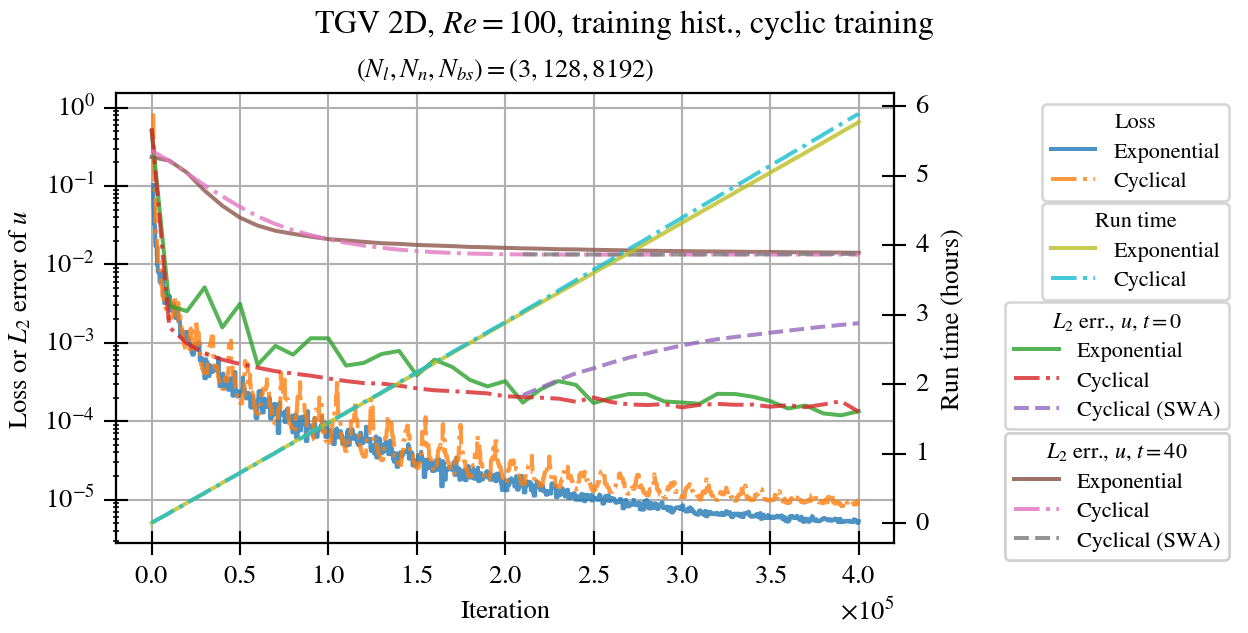
\includegraphics[width=\columnwidth]{tgv-2d-re100/pinn-nl3-nn128-npts8192-convergence}%
    \caption{%
        Training convergence history of 2D TGV $Re=\num{100}$ w/ PINN.
        $(N_l, N_n, N_{bs})=(3, 128, 8192)$.
    }
    \label{fig:tgv-pinn-loss}%
\end{figure}

\begin{figure}
    \centering%
    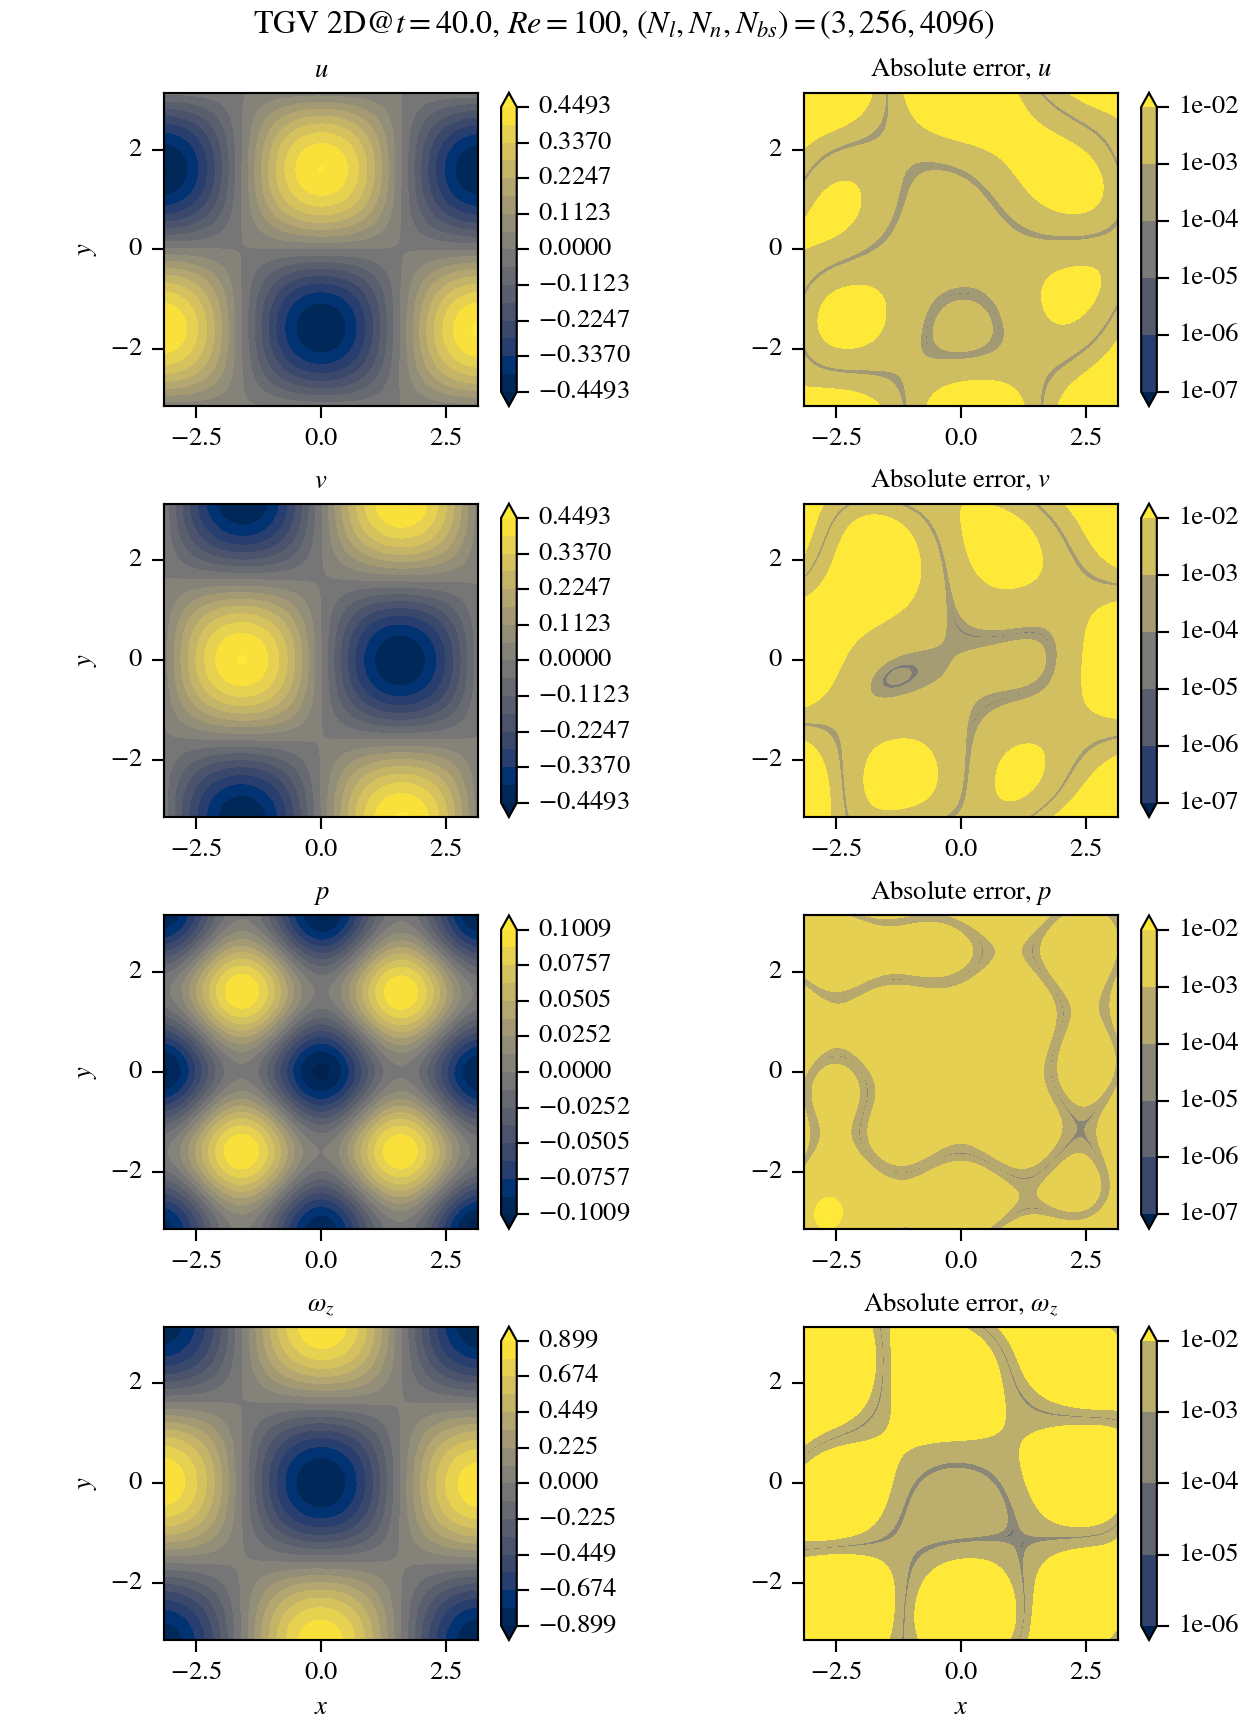
\includegraphics[width=\columnwidth]{tgv-2d-re100/pinn-nl3-nn256-npts4096-contours.png}
    \caption{%
        Contours of 2D TGV $Re=\num{100}$ using the PINN solver at $t=40$.
    }
    \label{fig:tgv-pinn-contours}%
\end{figure}

After training, the PINN solver's prediction errors (i.e., accuracy) were evaluated on cell centers of a $512$ $\times$ $512$ Cartesian mesh and at $t=0$, $2$, $4$, $\cdots$, $100$.
Figure \ref{fig:tgv-pinn-loss} shows the histories of the total loss and $L_2$ errors at $t=0$ and $t=40$ of the $u$ velocity on the left vertical axis.
The same figure also shows the run time (wall time) on the right vertical axis.
The total loss converges to around \num{1e-6}, which may be due to the single-precision floats used in PyTorch.
The errors at $t=0$ and $t=40$ converge to \num{1e-4} and \num{1e-2}, respectively.
We consider this to be reasonable because the net prediction errors for all $t\in[0, 100]$ is likely to be around \num{1e-3}, which is the square root of the total loss.
Note that because we also feed initial conditions for training ($L_4$ to $L_6$), so it is reasonable to see the prediction at $t=0$ performs better than later times.

Though the computational performance is not the focus of this paper, we would like to point out that the PINN solver took about 6 hours to converge with a V100 GPU, PetIBM only needed less than 10 seconds to get an error level of \num{1e-2} with a K40 GPU (and most of the time was overhead to initialize the solver).

In sum, we determined the PINN solver verified though the accuracy and the computational cost were not satisfying.
The low accuracy might be caused by the use of single-precision floats rather than implementation errors.
Figure \ref{fig:tgv-pinn-contours} shows the contours of the PINN solver's predictions.

% vim:ft=tex: